\documentclass[a4paper, 12pt]{article}
\usepackage[utf8]{inputenc}
\usepackage{url}
\usepackage{amsmath, amssymb, amsfonts}
\usepackage{graphicx}

\begin{document}
\begin{center}
{\LARGE \bf Praktikum Wissenschaftliches Rechnen \\ \vspace{0.2cm} (CFD, Final Project)}\\
\vspace{0.6cm}
{\small Group 9: Breznik, E., Cheng, Z., Ni, W., Schmidbartl, N.}
\end{center}
\normalfont
\section{The Topic}
For the final project, our group chose to extend the Navier Stokes code to be used in 3D for arbitrary geometries, with the ability of handling 
the Free Surface flow scenarios.
We put a lot of attention to designing a code that will work in 3D for as many different scenarios as possible. That is why we did not code a
special set of boundaries for just a few more known and frequently simulated situations, but rather made them completely dependent on the input 
geometry file.  

TODO:comment on not doing free surface
\subsection{Input}
The parameter file that was used as input in our previous worksheets remained, with just slight changes due to the additional dimension.
Only notable difference is, that we now take as an input also a scalar $velIN$, and a vector $velMW$. First one represent the velocity at the
inflow boundaries, and the second one the wall velocity for the moving wall boundaries. %TODO: when describin these b.c. say more about the velocity, what it represents

To make our code able to handle truly arbitrary scenarios, we designed so that it allows for any sort of implemented boundary conditions to be employed in any
domain cell - so even the obstacles inside the domain can have arbitrary boundaries, as opposed to only allowing that on the domain walls (as in workseet 3).
The standard boundary conditions, that we implemented, are 
\begin{itemize}
\item no slip,
\item free slip,
\item inflow,
\item outflow,
\item moving wall.
\end{itemize}
To specify, where which of them is applied, we used special numbering of cells when generating our input pgm files, which can be seen from table
\ref{tab1}, so our geometries are represented by a grayscale image with 7 levels of brightness.
\begin{table}
\centering
\label{tab1}
\begin{tabular}{|l|c|}
\hline
{\bf Cell type} & {\bf Number code}\\
\hline
water & 0 \\
air & 1 \\
no-slip & 2 \\
free-slip & 3 \\
inflow & 4 \\
outflow & 5 \\
moving wall & 6 \\
\hline
\end{tabular}
\caption{Number representations of different possible cell types.}
\end{table}
Since we are working in three dimensions, this image consists of a sequence of 2D ($xy$ plane) images. The orientation of coordinate system and an 
example picture for a small lid driven cavity case can be seen on figure \ref{fig1}. One geometry picture set thus needs to contain  
$(imax+2)\times(jmax+2)\times(kmax+2)$ numbers in $(jmax+2)\times(kmax+2)$ rows, and is typically very big.
\begin{figure}[hb!]
\centering
\label{fig1}
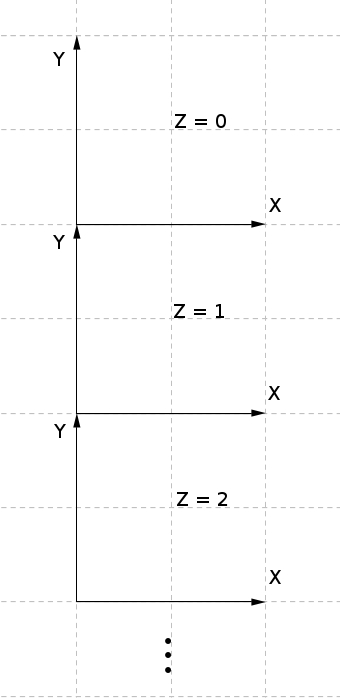
\includegraphics[height=5.8cm]{coord.jpg}
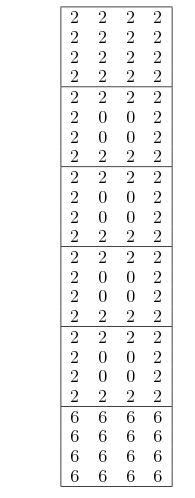
\includegraphics[height=5.8cm]{cavity2.jpg}

\includegraphics[height=5.65cm]{cavity20202.jpg}
\caption{The structure of our input pgm files and a lid driven cavity example case.}
\end{figure}


\section{Implementation}

\section{Problems, current state and future work}

\section{Results}

\begin{thebibliography}{99}
\bibitem{Griebel}
Griebel, M., Dornsheifer, T., Neunhoeffer, T.: \emph{Numerical Simulation in 
Fluid Dynamics: A Practical Introduction}. SIAM, {\bf 1998}.

\bibitem{Hirt}
Hirt, C. W., Nichols, B. D.: \emph{Volume of Fluid Method for the Dynamics of Free Boundaries}. Journal of Computational Physics {\bf 39} (1981).

\bibitem{sola}
Hirt, C. W., Nichols, B. D., Hotchkiss, R. S.: \emph{SOLA-VOF: A solution Algorithm for Transient Fluid Flow with Multiple Free Boudaries}. LASL, {\bf 1980}. 
\end{thebibliography}

\end{document}
